\chapter[Isometric and non-isometric task identification]{Identification of isometric and non-isometric upper-limb tasks using HD-EMG}
\label{ch:p4}
\textbf{Published as:} 
Jordani\'c, M., Rojas-Mart\'inez, M., Ma\~nanas, M.A., Alonso J.F., Marateb H.R.
Identification of isometric and non-isometric upper-limb tasks using HD-EMG 
\textit{Revista Iberoamericana de Autom\'atica e Inform\'atica industrial (RIAI)}, Accepted for publication, 2017

doi: ------------------

Impact Factor: 0.390; Position: 57 of 60 (Q4) AUTOMATION AND CONTROL SYSTEMS; 25 OF 26 (Q4) ROBOTICS.


\textbf{Abstract:} Identification of tasks and estimation of volitional movement based on electromyography (EMG) constitute a known problem that involves different areas in the field of expert systems and particularly pattern recognition, with many possible applications in assistive and rehabilitation devices. The obtained information can be very useful to control exoskeletons or robots used in active rehabilitation processes. The emerging method of high-density electromyography (HD-EMG) opens up new possibilities to extract neural information, and it has already been reported that the spatial distribution of HD-EMG intensity maps is a valuable feature in the identification of isometric tasks.

This study explores the use of the spatial distribution of myoelectric activity and carries out a task identification during dynamic exercises at different velocities which are much closer to the ones commonly used during therapy. To this end, HD-EMG signals were recorded in a group of healthy subjects while performing a set of isometric and dynamic upper limb tasks. The results show that spatial distribution is a very useful feature in the identification not only of isometric contractions but also of dynamic contractions, so it can be very useful to improve the control of rehabilitation devices, making it more natural and permitting to adapt better to the user.

\textbf{Keywords:}  bioengineering; electromyography; neuromuscular; rehabilitation

\section{Introduction}
Every year there are half of a million spinal cord injuries and 15 million strokes. These injuries can have an impact on the motor control, resulting in uncoordinated movements, lack of force, and spasticity. In these cases, robot-assisted therapies can be used to stimulate neuroplasticity \citep{vanPepen2004}. If the movement intention of the patient could be extracted in real time, it could be used to optimally control the assistive device based on the patient's state, maximizing the benefits of the therapy \citep{Hogan2006}.

The use of the spatial information of the myoelectric activation maps is a novel method that can achieve high results of task identification, both in healthy subjects \citep{Stango2015}, but also in patients with incomplete spinal cord injury \citep{Rojas-Martinez2013, Jordanic2016a, Jordanic2016b}. This study analyses the possibility of combining features extracted from these maps for the identification of set of isometric contractions performed at subjective force level, and also for the identification of dynamic contractions. Upper-limb motor tasks were recorded in a group of healthy subjects, and were consisted of hand movements in horizontal plane, involving mostly shoulder movements. These tasks were selected because they are usually in therapy with rehabilitation robots \citep{Badesa2014}.


\section{Methodology}

\subsection{Experimental protocol}
Five male subjects participated in the study (age: 24.8 $\pm$ 6.1 years, height: 178.6 $\pm$ 10.2 cm, weight: 76.8 $\pm$ 13.8 kg). They had no neuromuscular or musculoskeletal disorders of the upper limb prior to the recording. HD-EMG signals of \textit{biceps brachii}, \textit{triceps brachii}, \textit{pectoralis mayor}, and upper part of the \textit{trapezius} were recorded on the dominant side using two EMG amplifiers (EMG-USB, OT-Bioelettronica, Tur\'in, Italy) with synchronized sampling (2048 Hz sampling frequency). Using four 2D electrode arrays manufactured in our laboratory, 228 differential EMG channels were measured. Electrode arrays were designed as silver-plated eyelets embedded in the hydrophobic fabric with inter-electrode distance of 10 mm. Arrays were positioned so that the center of the array would follow the guidelines of the SENIAM project \citep{Hermens1999}.

Experimental protocol includes movements associated to the shoulder and is divided in two parts: a) recording of isometric contractions, and b) recording of dynamic contractions.
During the recording of the isometric contractions, subjects were seated upright with their back straight, elbow flexed at approximately 90 degrees, and shoulder in the neutral position (see figure \ref{fig:4-1}a). Maintaining this position, subjects performed three tasks, pushing a fixed object positioned directly in front of the subject forward, leftward, and rightward. Each of these tasks was realized at three different effort levels: low, medium, and high. Effort levels were chosen by the subject following his own perception of the exerted force. In addition, HD-EMG was also recorded during rest state. Each contraction had the duration of ten seconds with two minute rest period between contractions.

For recording of dynamic contractions, subjects were asked to maintain the previously described posture (straight back and elbow flexed at 90 degrees) and to displace an object over the horizontal plane, following the predefined trajectory (see figure \ref{fig:4-1}b):

\begin{enumerate}[a)]
\item From the center of the plane, located at approximately 30 cm in front of the subject, until the full extension of the shoulder, and return to the center.
\item From the center to the point located approximately 40 cm leftward, following the trajectory perpendicular to the previous one, and return to the center .
\item Finally repeat the same movement in the other direction, until the point located approximately 40 cm rightward, and return to the center.
\end{enumerate}

Each movement sequence was performed two times at two different velocities, fast and slow, based on the subject's perception, but without change in speed during each recording. Moreover, in addition to HD-EMG, positioning signal was also recorded. Proximity sensors were used and they would generate a signal each time the subject would reach one of the end-points of the trajectory (see figure \ref{fig:4-1}b).

\begin{figure*}[t!]
    \centering
    \begin{subfigure}[t]{0.45\textwidth}
        \centering
        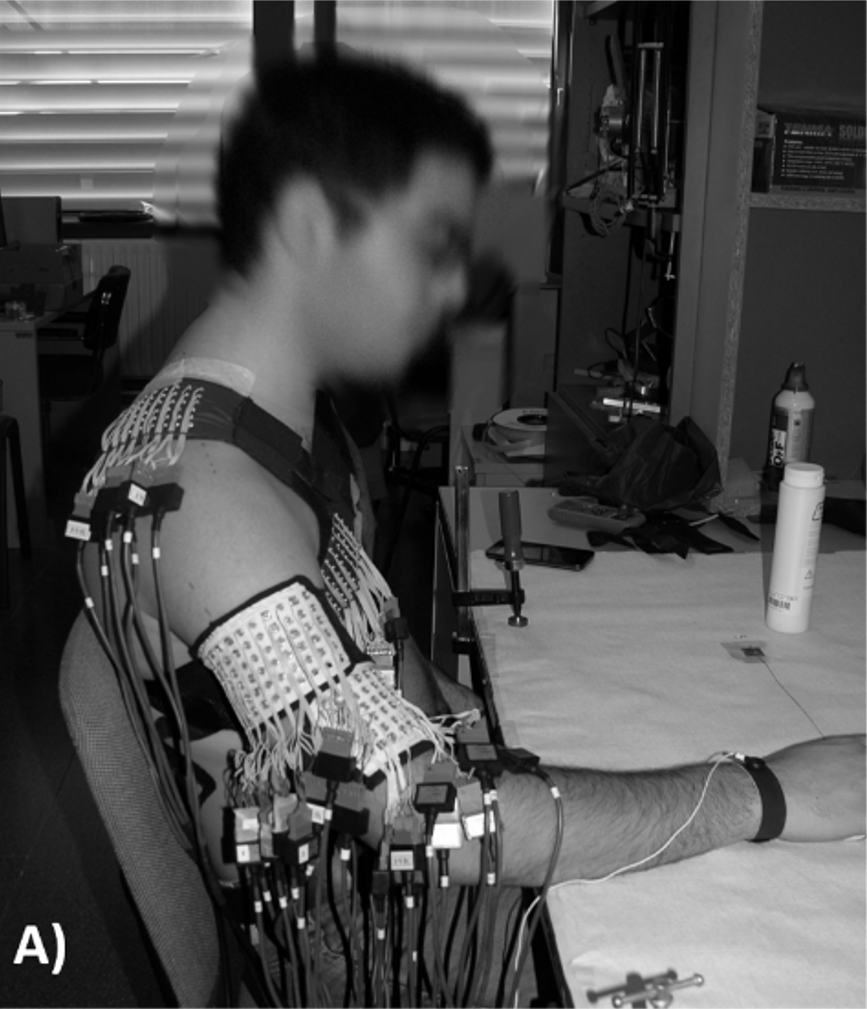
\includegraphics[height=2.9in]{Images/figure4_1a.png}
   
    \end{subfigure}%
    ~ 
    \begin{subfigure}[t]{0.45\textwidth}
        \centering
        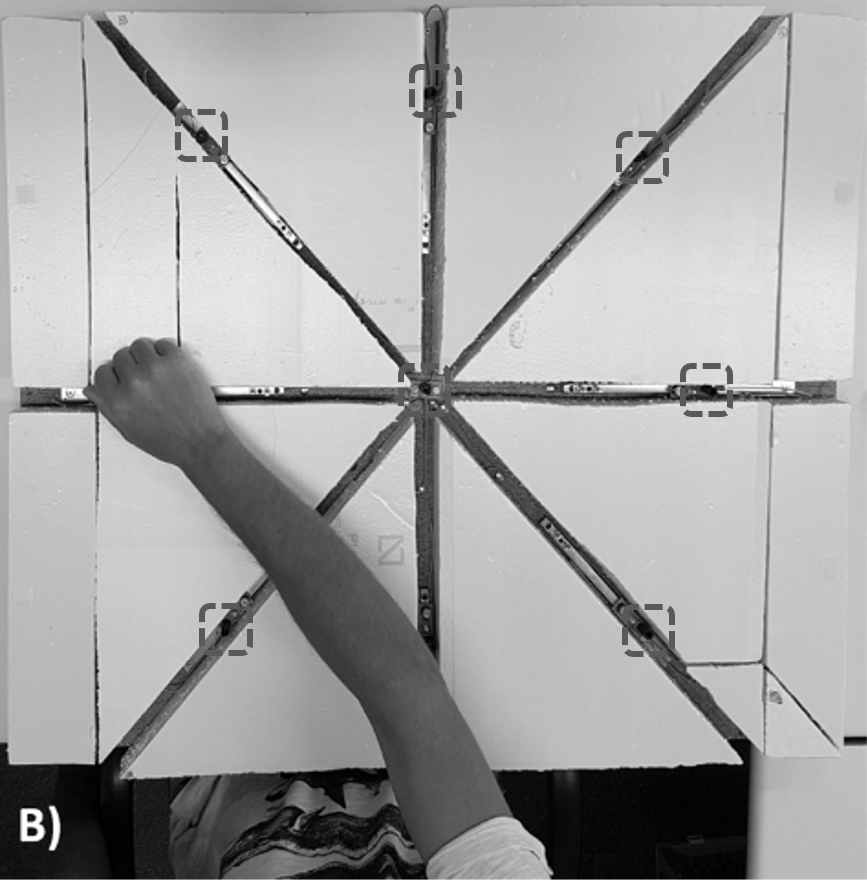
\includegraphics[height=2.9in]{Images/figure4_1b.png}
        
    \end{subfigure}
    \caption{Figure shows \textbf{A)} measurement equipment and the position of the subject during the experimental protocol, and \textbf{B)}experimental plane in which the tasks were performed. Position sensors are marked by dashed rectangles.}
\label{fig:4-1}
\end{figure*}


\subsection{Signal processing}
The recorded signals were recorded using 4\textsuperscript{th} order Butterworth filter with zero-phase. In addition, signals were filtered using an adaptive filter for reducing power line interference.

Afterwards, signals were divided in 250 ms time windows without overlapping and the RMS value was calculated for each channel. Using these values, activation map $HM$ was calculated for each time window as:
\begin{equation} \label{eq:4-1}
HM_{i,j} = \sqrt{\frac{\sum_n{sEMG_{i,j}^2 (n)}}{N}}
\end{equation}

, where $N=512$ samples (corresponding to time window of 250 ms), $i$ and $j$ are positions (row and column of the electrode array) of the sEMG channel, which corresponds to the position ($i,j$) of the pixel in the activation map $HM$. The channels identified as artifacts were substituted using triangle-based cubic interpolation \citep{Rojas-Martinez2012}.

From the activation maps, features were extracted: logarithm of the average intensity of the map (Ilog), and the center of gravity (CG). In the first case, it was already shown that the logarithmic transform is useful in the identification of effort level \citep{Rojas-Martinez2012}, and in the second case, it was shown that the spatial distribution of myoelectric activity changes with the force level \citep{Holtermann2005}, and with the isometric task intention \citep{Jordanic2016a}.

On the other hand, positioning signal recorded during dynamic part of the protocol was used to sort the HD-EMG signals to in order to obtain the segments corresponding to each of the movements described in the protocol.


\subsection{Movement classification}
The classification was realized for each subject individually both for the isometric tasks and for the dynamic tasks. For the isometric tasks, two types of the classification were considered:

\begin{enumerate}[a)]
\item identification of four tasks regardless of the effort level (rest, push forward, push leftward, push rightward)

\item identification of tasks and effort levels (identification of three tasks at three different effort levels, and rest state)
\end{enumerate}

The identification of isometric tasks was performed to validate the experimental protocol. Although in our previous work we managed to identify isometric tasks with high sensitivity and precision, using both intensity and spatial features, the tasks considered in that studies were related to the elbow, and not to the shoulder \citep{Jordanic2016a, Jordanic2016b, Rojas-Martinez2013}.

For the dynamic task, identification consisted of classification each of the following tasks:
 
\begin{enumerate}[a)]
\item moving forward
\item return back towards center
\item moving leftward
\item return back towards center
\item moving rightward
\item return back towards center
\end{enumerate}

For identification of task, classifier based on linear discriminant analysis (LDA) was used, a technique often used in myoelectric pattern recognition because of the speed and low computational complexity \citep{Zhou2007}.

In the case of isometric contractions, database was separated in two groups, training set, consisting of 60\% of the available data, and test set, consisting of 40\% of the available data. This data separation, followed by the training and testing of the classifier was repeated 100 times in order to minimize possible statistical error (hold-out validation method). The obtained identification results are the averaged result over 100 iterations.

In the case of dynamic contractions, classifier was trained using the observations recorded in one recording sequence (both for slow and fast movements), and validated using the observations recorded in the other sequence. Afterwards, the training set and the test set were swapped and the identification was repeated. The results are the averaged results of these two identifications. This type of validation was used to reduce the possible statistical error, although it is possible that in the second recording subject learned how to control the velocity and perform the exercise better.

Finally, the performance of the classification was expressed in terms of sensitivity (S) and precision (P) \citep{Farina2001}, calculated as:
\begin{equation}
S = \frac{TP}{VP+FN}
\end{equation}
\begin{equation}
S = \frac{VP}{VP+FP}
\end{equation}
, where TP is the number of true positives, that is, correctly classified samples, FP is the number of false positives, which indicate number of wrongly classified samples to a certain class, and FN is number of false negatives, that is, number of samples incorrectly classified to another class. The sensitivity (S) and precision (P) were obtained for each of the classes, and the averaged result was calculated.



\section{Results}

\subsection{Activation maps}
In the figure \ref{fig:4-2} activation maps of \textit{pectoralis mayor} are shown. Different activation patterns can be observed during the performance of dynamic tasks. It should be noted that the activation intensity varies depending on the exercise, presenting the highest activation (in mV) during the movements from full forward extension to the center of the plane, and the reverse. Also, it can be noted that the spatial distribution varies depending on the exercise, for example, during the contraction associated with the forward movement (see figure \ref{fig:4-2}a) activation is located at the left side of the map (columns 1 to 3), whereas in the rightward movement (see figure \ref{fig:4-2}b) the are with higher activity is located in the right part of the map (column 8, rows 2 to 4). Although only maps of \textit{pectoralis mayor} are shown, the similar differentiation can be found in the remaining three muscles and this information is used in the identification. 

\begin{figure}[ht]
\centering
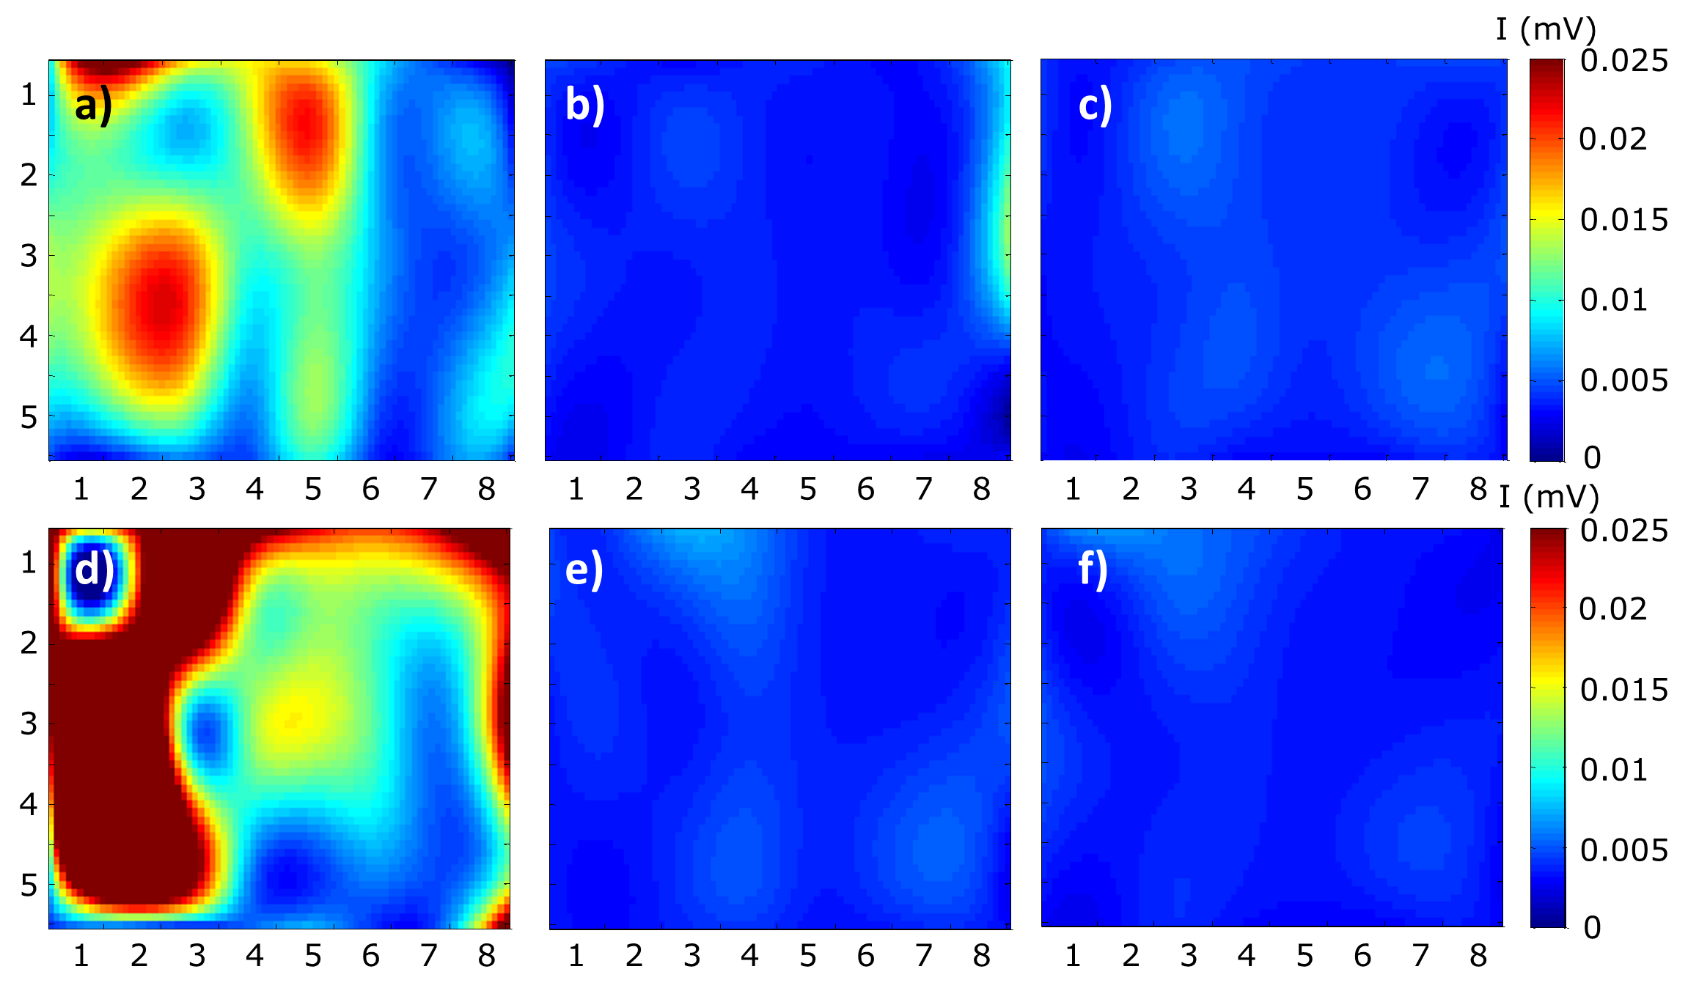
\includegraphics[width=0.99\textwidth]{Images/figure4_2.png}
\caption{Activation maps of \textit{pectoralis mayor} of one of the subjects. Up. Movement from central point a) forward, b) rightward, and c) leftward. Down. Movement toward center from  d) ahead, e) right, and f) left.}
\label{fig:4-2}
\end{figure}

\subsection{Isometric task identification}
With the objective to establish if the spatial distribution of intensity improves the identification, two types of identification were performed: the identification based only on intensity features, and the identification based on the combination of intensity and spatial features. Additionally, identification of task was performed (forward, rightward, leftward, and rest), and the identification of task and effort levels. Results of identification of tasks, regardless of effort level are shown in table \ref{tb:4-1}, whereas results of the identification of task and effort level are shown in the table \ref{tb:4-2}.

\begin{table}[]
\centering
\caption{Results of the identification of isometric tasks using the Ilog features and combination of Ilog and CG features. The results are presented as mean and standard deviation calculated across five subjects.}
\label{tb:4-1}
\begin{tabular}{llcccc}
 
              & \multicolumn{2}{c}{\textbf{Ilog}}                            & \multicolumn{2}{c}{\textbf{Ilog + CG}}                       \\
\textbf{Task} & \textbf{Sensitivity}     & \textbf{Precision}       & \textbf{Sensitivity}     & \textbf{Precision}       \\ \hline
                         &                                           &          &          &                   \\
Forward       & 73 $\pm$ 13              & 77.1 $\pm$ 15            & 92.1 $\pm$ 6.9           & 93.6 $\pm$ 6.4           \\
Rightward     & 83.5 $\pm$ 16            & 92 $\pm$ 9.4             & 96.2 $\pm$ 4.9           & 95.9 $\pm$ 3.9           \\
Leftward      & 85.8 $\pm$ 14            & 87.3 $\pm$ 13            & 96.1 $\pm$ 5.4           & 97.8 $\pm$ 5             \\
Rest          & 98.7 $\pm$ 2.1           & 87.1 $\pm$ 3.2           & 100 $\pm$ 0              & 98.5 $\pm$ 3.4           \\ 
\textbf{Mean} & \textbf{85.3 $\pm$ 11.2} & \textbf{85.9 $\pm$ 10.2} & \textbf{96.1 $\pm$  4.3} & \textbf{96.4  $\pm$ 4.7}
\end{tabular}
\end{table}

\begin{table}[]
\centering
\caption{Results of the identification of isometric tasks and effort levels using the Ilog features and combination of Ilog and CG features. The results are presented as mean and standard deviation calculated across five subjects.}
\label{tb:4-2}
\begin{tabular}{llcccc}
              & \multicolumn{2}{c}{\textbf{Ilog}}                            & \multicolumn{2}{c}{\textbf{Ilog + CG}}                       \\
\textbf{Task} & \textbf{Force} & \textbf{Sensitivity}                          & \textbf{Precision}                           & \textbf{Sensitivity}                         & \textbf{Precision}                          \\ \hline
              &                &                                               &                                              &                                             &                                             \\
              & low            & 91.4 $\pm$ 14                                 & 89.8 $\pm$ 12                                & 99 $\pm$ 2.3                                & 99.2 $\pm$ 1.7                              \\
Forward       & medium         & 86.4 $\pm$ 25                                 & 88.8 $\pm$ 16                                & 96.7 $\pm$ 7.5                              & 99.4 $\pm$ 1.4                              \\
              & high           & 87.7 $\pm$ 14                                 & 89.9 $\pm$ 14                                & 95.8 $\pm$ 6                                & 98.5 $\pm$ 3.4                              \\ \hline
              & low            & 98.3 $\pm$ 3.7                                & 89.4 $\pm$ 11                                & 97.7 $\pm$ 3.6                              & 94.6 $\pm$ 7.5                              \\
Rightward     & medium         & 90.4 $\pm$ 18                                 & 91.3 $\pm$ 6.5                               & 98.3 $\pm$ 3.7                              & 98.3 $\pm$ 3.9                              \\
              & high           & 98.3 $\pm$ 3.9                                & 100 $\pm$ 0                                  & 100 $\pm$ 0                                 & 99.2 $\pm$ 1.7                              \\ \hline
              & low            & 96 $\pm$ 5.1                                  & 92.1 $\pm$ 8.3                               & 96.9 $\pm$ 7                                & 95.2 $\pm$ 7.3                              \\
Leftward      & medium         & 85.7 $\pm$ 5.9                                & 85.3 $\pm$ 11                                & 94.4 $\pm$ 7.8                              & 94.8 $\pm$ 7.4                              \\
              & high           & 93.9 $\pm$ 7.1                                & 96 $\pm$ 7.2                                 & 98.3 $\pm$ 3.7                              & 97 $\pm$ 6.6                                \\ \hline
Rest          &                & \multicolumn{1}{l}{97.5 $\pm$ 5.6}            & \multicolumn{1}{l}{98.5 $\pm$ 3.4}           & \multicolumn{1}{l}{100 $\pm$ 0}             & \multicolumn{1}{l}{99 $\pm$ 2.2}            \\
\textbf{Mean} & \textbf{}      & \multicolumn{1}{l}{\textbf{92.6  $\pm$ 10.2}} & \multicolumn{1}{l}{\textbf{92.1  $\pm$ 8.9}} & \multicolumn{1}{l}{\textbf{97.7 $\pm$ 4.2}} & \multicolumn{1}{l}{\textbf{97.5 $\pm$ 4.3}}
\end{tabular}
\end{table}

It can be seen that by adding center of gravity to intensity features, results improve for approximately 10\% in the case of task identification and 5\% in the case of identification of task and effort level. Moreover, when using center of gravity, standard deviation is smaller. Therefore, spatial distribution has a positive effect on the identification.


\subsection{Dynamic task identification}
In the case of dynamic task identification, 6 classes are considered: move forward and return, move leftward and return, and move rightward and return.

Tables \ref{tb:4-3} and \ref{tb:4-4} show the results obtained by averaging results of each patient, using only intensity features (table \ref{tb:4-3}), and combination of intensity and spatial features (table \ref{tb:4-4}). As in isometric contractions, identification results are higher when combining intensity and spatial features.

\begin{table}[]
\centering
\caption{Identification of six dynamic contractions based on the intensity features separately for slow movements and fast movements. The results are presented as mean and standard deviation calculated across five subjects.}
\label{tb:4-3}
\begin{tabular}{llcccc}
                   &           & \multicolumn{2}{c}{\textbf{Slow}}          & \multicolumn{2}{c}{\textbf{Fast}}           \\
                   &           & \textbf{Sensitivity} & \textbf{Precision}  & \textbf{Sensitivity} & \textbf{Precision}   \\ \hline
                   &           &                      &                     &                      &                      \\
From the center    & Leftward  & 60.7 $\pm$ 12.6          & 68.8 $\pm$ 7.9          & 77.2 $\pm$ 14.1          & 74.9 $\pm$ 13.5          \\
                   & Rightward & 87.7 $\pm$ 7.8           & 79.6 $\pm$ 8.7          & 77.2 $\pm$ 14.3          & 75.7 $\pm$ 12.0          \\
                   & Forward   & 77.9 $\pm$ 9.9           & 74.8 $\pm$ 10.1         & 76.8 $\pm$ 13.6          & 77.0 $\pm$ 10.6          \\ \hline
Toward center from & Ahead     & 73.4 $\pm$ 11.8          & 74.7 $\pm$ 11.1         & 80.4 $\pm$ 14.2          & 75.5 $\pm$ 9.5           \\
                   & Right     & 68.8 $\pm$ 11.5          & 75.7 $\pm$ 12.1         & 85.4 $\pm$ 9.3           & 78.8 $\pm$ 10.4          \\
                   & Forward   & 71.8 $\pm$ 9.0           & 72.9 $\pm$ 8.3          & 78.3 $\pm$ 20.9          & 71.9 $\pm$ 15.6          \\ \hline
\textbf{Mean}      & \textbf{} & \textbf{73.4 $\pm$ 10.4} & \textbf{74.4 $\pm$ 9.7} & \textbf{79.2 $\pm$ 14.4} & \textbf{75.7 $\pm$ 11.9}
\end{tabular}
\end{table}


\begin{table}[]
\centering
\caption{Identification of six dynamic contractions based on the combination of intensity and spatial features separately for slow movements and fast movements. The results are presented as mean and standard deviation calculated across five subjects.}
\label{tb:4-4}
\begin{tabular}{llcccc}
                   &           & \multicolumn{2}{c}{\textbf{Slow}}           & \multicolumn{2}{c}{\textbf{Fast}}           \\
                   &           & \textbf{Sensitivity} & \textbf{Precision}   & \textbf{Sensitivity} & \textbf{Precision}   \\ \hline
                   &           & \multicolumn{1}{l}{} & \multicolumn{1}{l}{} & \multicolumn{1}{l}{} & \multicolumn{1}{l}{} \\
From the center    & Leftward  & 85.0 $\pm$ 13.1          & 83.1 $\pm$ 5.7           & 94.4 $\pm$ 11.4          & 94.0 $\pm$ 13.3          \\
                   & Rightward & 94.8 $\pm$ 3.4           & 91.9 $\pm$ 7.9           & 95.6 $\pm$ 9.2           & 90.6 $\pm$ 14.6          \\
                   & Forward   & 84.4 $\pm$ 11.0          & 86.7 $\pm$ 11.0          & 95.4 $\pm$ 9.2           & 90.4 $\pm$ 13.8          \\ \hline
Toward center from & Ahead     & 92.3 $\pm$ 7.1           & 92.4 $\pm$ 12.8          & 93.7 $\pm$ 14.1          & 93.7 $\pm$ 14.1          \\
                   & Right     & 85.1 $\pm$ 6.2           & 86.7 $\pm$ 6.6           & 96.6 $\pm$ 7.1           & 92.1 $\pm$ 12.1          \\
                   & Forward   & 81.0 $\pm$ 5.6           & 89.7 $\pm$ 7.4           & 91.8 $\pm$ 11.0          & 85.5 $\pm$ 14.0          \\ \hline
\textbf{Mean}      & \textbf{} & \textbf{87.1 $\pm$ 7.7}  & \textbf{88.4 $\pm$ 8.6}  & \textbf{94.6 $\pm$ 10.3} & \textbf{91.0 $\pm$ 13.6}
\end{tabular}
\end{table}

Higher variability can be observed compared to the isometric task identification, as well as lower sensitivity and precision, as could be expected since the dynamic contractions represent a more complex problem. Finally, it should be noted that although the mean identification results of fast movements are higher than slow movements, the variability is higher in identification of fast movements. Therefore, it can not be said with certainty that fast movements can be identified with higher identification results.


\section{Conclusions}
En todos los casos se ha comprobado que los mejores resultados se obtienen cuando la clasificación tiene en cuenta tanto la intensidad en escala logarítmica como el centro de gravedad de los mapas de activación muscular. Este hecho indica que existe una interdependencia entre la distribución espacial de la intensidad y la tarea desarrollada tanto en contracciones isométricas como en dinámicas. Al incluir una característica relacionada con la distribución espacial de las unidades motoras no solo mejoran los índices en promedio, sino que además disminuye ostensiblemente su desviación estándar por lo que se puede concluir que este método añade robustez al análisis.

Estos resultados concuerdan con los presentados en diferentes estudios (Hargrove et al. 2007; Farina et al. 2008; Jordanic et al. 2016b; Zhou et al. 2007) y pueden estar relacionados con la compartimentación neuromuscular que indica que hay regiones con actividad funcional diferenciada dentro de un mismo músculo. Por lo tanto, es posible que estos hallazgos puedan extenderse al músculo Pectoralis Major que no había sido evaluado previamente en nuestros estudios anteriores.

Otro factor a destacar es que, en el caso de contracciones isométricas, no solo se puede obtener información acerca de la dirección de la contracción (frente, derecha o izquierda) sino también del nivel de fuerza ejercido, lo que permitiría controlar simultáneamente tanto la dirección del movimiento como la fuerza deseada lo cual es de gran importancia en el caso de querer controlar un dispositivo externo de manera más natural. 

En el caso de las contracciones dinámicas el rendimiento de la clasificación es más bajo ya que por la naturaleza propia de la señal obtenida y de la contracción (que implica movimiento de la articulación) hace que la diferenciación resulte más compleja que en el caso de los ejercicios isométricos donde no hay movimiento de la articulación. Además, en este estudio se quiso evaluar un movimiento totalmente voluntario, permitiendo al paciente regular la velocidad del mismo en cada trayecto, lo que también aumenta la complejidad del análisis. Este caso se acerca más a las condiciones reales de movimiento que se esperan durante la terapia robótica. Sin embargo, los resultados obtenidos son prometedores (sensibilidad y precisión cercanas al 90\%) y se deben investigar otro tipo de características espaciales con el fin de mejorar el rendimiento y hacer la clasificación más robusta.

Por otro lado, los resultados globales para las contracciones a ritmo rápido y lento son similares, ya que, aunque en promedio para los primeros se obtiene un mayor valor, la variabilidad es alta (>10\%). Por tanto, no se puede concluir con seguridad si el rendimiento de la identificación depende de la velocidad de movimiento. A este respecto sería necesario contar con una base de datos mayor para poder extraer una conclusión.

Como conclusión general, se ha demostrado que la metodología propuesta y los resultados obtenidos son prometedores y cabe la posibilidad de añadir la información extraída de señales HD-EMG al lazo de control de dispositivos externos como sistemas robóticos para rehabilitación donde se quiera tener en cuenta la intención voluntaria del paciente.
 En trabajos futuros, se extenderá el protocolo y la metodología desarrollada al estudio de pacientes con alteraciones neuromusculares basándose en características asociadas a la intensidad y distribución espacial de mapas de activación HD-EMG. Esto con el fin de controlar dispositivos de asistencia en terapias de rehabilitación.
 
 \section{Acknowledgments}
 The authors are grateful to Ignasi Gallardo for his collaboration in the design of the study.
 
 This work has been partially supported by the project ROBERT of the CIBER-BBN, and by the Spanish Ministry of Economy and Competitiveness (project DPI2014-59049-R).

